% Options for packages loaded elsewhere
\PassOptionsToPackage{unicode}{hyperref}
\PassOptionsToPackage{hyphens}{url}
%
\documentclass[
]{rescience}
\usepackage{lmodern}
\usepackage{amssymb,amsmath}
\usepackage{ifxetex,ifluatex}
\ifnum 0\ifxetex 1\fi\ifluatex 1\fi=0 % if pdftex
  \usepackage[T1]{fontenc}
  \usepackage[utf8]{inputenc}
  \usepackage{textcomp} % provide euro and other symbols
\else % if luatex or xetex
  \usepackage{unicode-math}
  \defaultfontfeatures{Scale=MatchLowercase}
  \defaultfontfeatures[\rmfamily]{Ligatures=TeX,Scale=1}
\fi
% Use upquote if available, for straight quotes in verbatim environments
\IfFileExists{upquote.sty}{\usepackage{upquote}}{}
\IfFileExists{microtype.sty}{% use microtype if available
  \usepackage[]{microtype}
  \UseMicrotypeSet[protrusion]{basicmath} % disable protrusion for tt fonts
}{}
\makeatletter
\@ifundefined{KOMAClassName}{% if non-KOMA class
  \IfFileExists{parskip.sty}{%
    \usepackage{parskip}
  }{% else
    \setlength{\parindent}{0pt}
    \setlength{\parskip}{6pt plus 2pt minus 1pt}}
}{% if KOMA class
  \KOMAoptions{parskip=half}}
\makeatother
\usepackage{xcolor}
\IfFileExists{xurl.sty}{\usepackage{xurl}}{} % add URL line breaks if available
\IfFileExists{bookmark.sty}{\usepackage{bookmark}}{\usepackage{hyperref}}
\hypersetup{
  pdftitle={Reproducing ``Fluctuation Domains''},
%  hidelinks,
  pdfcreator={LaTeX via pandoc}}
\urlstyle{same} % disable monospaced font for URLs
\usepackage{color}
\usepackage{fancyvrb}
\newcommand{\VerbBar}{|}
\newcommand{\VERB}{\Verb[commandchars=\\\{\}]}
\DefineVerbatimEnvironment{Highlighting}{Verbatim}{commandchars=\\\{\}}
% Add ',fontsize=\small' for more characters per line
\usepackage{framed}
\definecolor{shadecolor}{RGB}{248,248,248}
\newenvironment{Shaded}{\begin{snugshade}}{\end{snugshade}}
\newcommand{\AlertTok}[1]{\textcolor[rgb]{0.94,0.16,0.16}{#1}}
\newcommand{\AnnotationTok}[1]{\textcolor[rgb]{0.56,0.35,0.01}{\textbf{\textit{#1}}}}
\newcommand{\AttributeTok}[1]{\textcolor[rgb]{0.77,0.63,0.00}{#1}}
\newcommand{\BaseNTok}[1]{\textcolor[rgb]{0.00,0.00,0.81}{#1}}
\newcommand{\BuiltInTok}[1]{#1}
\newcommand{\CharTok}[1]{\textcolor[rgb]{0.31,0.60,0.02}{#1}}
\newcommand{\CommentTok}[1]{\textcolor[rgb]{0.56,0.35,0.01}{\textit{#1}}}
\newcommand{\CommentVarTok}[1]{\textcolor[rgb]{0.56,0.35,0.01}{\textbf{\textit{#1}}}}
\newcommand{\ConstantTok}[1]{\textcolor[rgb]{0.00,0.00,0.00}{#1}}
\newcommand{\ControlFlowTok}[1]{\textcolor[rgb]{0.13,0.29,0.53}{\textbf{#1}}}
\newcommand{\DataTypeTok}[1]{\textcolor[rgb]{0.13,0.29,0.53}{#1}}
\newcommand{\DecValTok}[1]{\textcolor[rgb]{0.00,0.00,0.81}{#1}}
\newcommand{\DocumentationTok}[1]{\textcolor[rgb]{0.56,0.35,0.01}{\textbf{\textit{#1}}}}
\newcommand{\ErrorTok}[1]{\textcolor[rgb]{0.64,0.00,0.00}{\textbf{#1}}}
\newcommand{\ExtensionTok}[1]{#1}
\newcommand{\FloatTok}[1]{\textcolor[rgb]{0.00,0.00,0.81}{#1}}
\newcommand{\FunctionTok}[1]{\textcolor[rgb]{0.00,0.00,0.00}{#1}}
\newcommand{\ImportTok}[1]{#1}
\newcommand{\InformationTok}[1]{\textcolor[rgb]{0.56,0.35,0.01}{\textbf{\textit{#1}}}}
\newcommand{\KeywordTok}[1]{\textcolor[rgb]{0.13,0.29,0.53}{\textbf{#1}}}
\newcommand{\NormalTok}[1]{#1}
\newcommand{\OperatorTok}[1]{\textcolor[rgb]{0.81,0.36,0.00}{\textbf{#1}}}
\newcommand{\OtherTok}[1]{\textcolor[rgb]{0.56,0.35,0.01}{#1}}
\newcommand{\PreprocessorTok}[1]{\textcolor[rgb]{0.56,0.35,0.01}{\textit{#1}}}
\newcommand{\RegionMarkerTok}[1]{#1}
\newcommand{\SpecialCharTok}[1]{\textcolor[rgb]{0.00,0.00,0.00}{#1}}
\newcommand{\SpecialStringTok}[1]{\textcolor[rgb]{0.31,0.60,0.02}{#1}}
\newcommand{\StringTok}[1]{\textcolor[rgb]{0.31,0.60,0.02}{#1}}
\newcommand{\VariableTok}[1]{\textcolor[rgb]{0.00,0.00,0.00}{#1}}
\newcommand{\VerbatimStringTok}[1]{\textcolor[rgb]{0.31,0.60,0.02}{#1}}
\newcommand{\WarningTok}[1]{\textcolor[rgb]{0.56,0.35,0.01}{\textbf{\textit{#1}}}}
\usepackage{graphicx}
\makeatletter
\def\maxwidth{\ifdim\Gin@nat@width>\linewidth\linewidth\else\Gin@nat@width\fi}
\def\maxheight{\ifdim\Gin@nat@height>\textheight\textheight\else\Gin@nat@height\fi}
\makeatother
% Scale images if necessary, so that they will not overflow the page
% margins by default, and it is still possible to overwrite the defaults
% using explicit options in \includegraphics[width, height, ...]{}
\setkeys{Gin}{width=\maxwidth,height=\maxheight,keepaspectratio}
% Set default figure placement to htbp
\makeatletter
\def\fps@figure{htbp}
\makeatother
\setlength{\emergencystretch}{3em} % prevent overfull lines
\providecommand{\tightlist}{%
  \setlength{\itemsep}{0pt}\setlength{\parskip}{0pt}}
\setcounter{secnumdepth}{-\maxdimen} % remove section numbering

\title{Reproducing ``Fluctuation Domains''}
%\author{}
%\date{}

\begin{document}
\maketitle

%% ----------------------------------------------------------------------------
%% ReScience article template
%% Copyright (c) 2018 N.P. Rougier,
%% Released under a Creative Commons Attribution 4.0 International license.
%% ----------------------------------------------------------------------------

%% --- Top left header --------------------------------------------------------
\begin{tikzpicture}[remember picture, overlay]
  \node [shape=rectangle, draw=darkred, fill=darkred, yshift=-34mm,
        anchor=north west, minimum width=3.75cm, minimum height=10mm]
        at (current page.north west) {};
  \node [text=white, anchor=center, yshift=-39mm, xshift=1.875cm]
         at (current page.north west) {\small \SpaceRoboto RESCIENCE C};
\end{tikzpicture}


%% --- Title -------------------------------------------------------------------
{\let\newpage\relax\maketitle} \maketitle


%% --- Margin information -----------------------------------------------------
\marginnote{
  \footnotesize \sffamily
  \textbf{Edited by}\\
  \ifdefempty{\editorNAME}{\textcolor{darkgray}{(Editor)}}
             {\editorNAME\ifdefempty{\editorORCID}{}{$^{\orcid{\editorORCID}}$}}\\
  ~\\
  %%
  \ifdefempty{\reviewerINAME}{}
  {
  \textbf{Reviewed by}\\
  \ifdefempty{\reviewerINAME}{\textcolor{darkgray}{}}
             {\reviewerINAME\ifdefempty{\reviewerIORCID}{}{$^{\orcid{\reviewerIORCID}}$}\\}
  \ifdefempty{\reviewerIINAME}{\textcolor{darkgray}{}}
             {\reviewerIINAME\ifdefempty{\reviewerIIORCID}{}{$^{\orcid{\reviewerIIORCID}}$}\\}
  ~\\
  }
  %%
  \textbf{Received}\\
  \ifdefempty{\dateRECEIVED}{---}{\dateRECEIVED}\\
  ~\\
  %%
  \textbf{Published}\\
  \ifdefempty{\datePUBLISHED}{---}{\datePUBLISHED}\\
  ~\\
  %%
  \textbf{DOI}\\
  \ifdefempty{\articleDOI}{---}{\articleDOI}
}


%% --- Bottom statement -------------------------------------------------------
\newcommand{\container}[1]{\def\@container{#1}}
\begin{container}
  \afterpage {
    \begin{statement}
      \scriptsize \sffamily
      \hrule \vskip .5em
      Copyright © \articleYEAR~\authorsABBRV,
      released under a Creative Commons Attribution 4.0 International license.

      Correspondence should be addressed to
      \contactNAME~(\href{mailto:\contactEMAIL}{\contactEMAIL})

      The authors have declared that no competing interests exists.

      \ifdefempty{\codeURL}{}
      {Code is available at
      \href{\codeURL}{\detokenize\expandafter{\codeURL}}\ifdefempty{\codeDOI}{.}{ -- DOI \doi{\codeDOI}.}\ifdefempty{\codeSWH}{.}{ -- SWH  \href{https://archive.softwareheritage.org/\codeSWH/}{\detokenize\expandafter{\codeSWH}}.}}

      \ifdefempty{\dataURL}{}
      {Data is available at
      \href{\dataURL}{\detokenize\expandafter{\dataURL}}\ifdefempty{\dataDOI}{.}{ -- DOI \doi{\dataDOI}.}}

      \ifdefempty{\reviewURL}{}
     {Open peer review is available at \href{\reviewURL}{\detokenize\expandafter{\reviewURL}}.}
    \end{statement}
  }
\end{container}


%% --- Abstract ---------------------------------------------------------------
 \ifdefempty{\articleABSTRACT}{}{
   {\small \sffamily \textbf{Abstract} \articleABSTRACT \par}
 }


%% --- Replication ------------------------------------------------------------
 \ifdefempty{\replicationBIB}{}{
   {\small \sffamily \bfseries A replication of}
   \ifdefempty{\replicationURL}
        {\href{http://doi.org/\replicationDOI}{\small \sffamily \replicationBIB}}
        {\href{\replicationURL}{\small \sffamily \replicationBIB}}.
 \par }

\hypertarget{historical-context}{%
\subsection{Historical context}\label{historical-context}}

In this analysis I seek to reproduce the numerical results of (Boettiger,
Dushoff, and Weitz 2010), which focuses on the evolutionary trajectory
of species trait under selection, as predicted by the so-called
``Canonical Equation'' of adaptive dynamics (Dieckmann and Law 1996).
Theoretical work I present in the paper predicts the emergence of a
`flutation enhancement' regime far from an evolutionary stable point,
and suggests that the evolution of traits which start in this distant
region would deviate substantially from the expected evolutionary path
predicted by the canonical equation. In particular, the distribution of
such trajectories could be bimodal, making the ``canonical'' path far
from the most likely path. The details of this distribution cannot be
solved for analytically however, so in this paper I resorted to an
replicate exact stochastic simulations of the evolutionary model using a
Gillespie algorithm (Gillespie 1977).

I implemented Gillespie algorithm for the evolutionary model in C code,
and wrapped the C code in an R package structure to make it easier to
run and easier to plot results. The C code depended on one standard C
library, the GNU Scientific Library, which has evolved considerably
(with one major version change) since that time. The original source
code was `published' (initially only on a colleague's website, as stated
in the paper, though later copies were submitted to formal archives, as
discussed below). That original copy was distributed under a GPL v3
licence, though I later replaced that with a CC0 license when submitting
the version to a data archive (Dryad) which required public domain
declarations.

\hypertarget{retrieval-of-software}{%
\subsection{Retrieval of software}\label{retrieval-of-software}}

I have changed laptops and the organizational schemes I use for my
documents several times since publishing the original paper. Though I
still have my original copy of the code for the manuscript sitting
around somewhere in a compressed, encrypted archive blob that now lives
on Amazon Glacier, accessing it there would have been complex and
demanding. Fortunately, in 2011 I uploaded a copy of this code to a
dedicated repository on GitHub at
\url{https://github.com/cboettig/fluctuationDomains}. I rely on this
copy for the remainder of this reproducibility effort.

The published paper itself states that the code is available at the
personal website of one of my co-authors, with URL
\url{http://ecotheory.biology.gatech.edu/downloads/}. Fortunately, this
URL still resolves (my colleague is still at the same institution), and
does indeed contain a downloadable zip file with a copy of the code. In
2012, I had uploaded a copy of this code as a supplement to Dryad, but
both on my CV at the time and on my colleague's website we had recorded
only the Dryad handle URL,
\url{http://datadryad.org/handle/10255/dryad.37625}, which no longer
resolves. That handle can be resolved by the WayBackMachine, which
doesn't contain the code archive but does reveal the DOI,
\url{http://dx.doi.org/10.5061/dryad.j8n0p7vc}, which successfully
resolves to the Dryad copy. The code can also be found by searching the
Dryad web interface for my surname (though it is listed as ``data'' and
not ``software.'' In 2017, I had also imported the GitHub copy into the
Zenodo data repository where it was again assigned a DOI and is
identified as software in the metadata. I note that the package was
never submitted to the Central R Archive Network, CRAN.

Notably, these versions are not entirely the same. The
GitHub/Zenodo/Dryad version has the addition of a \texttt{configure.ac}
script for autoconf, intended to make the package more portable in
assisting with the linkage to the GSL library, which is missing from the
original deposit (on the GeorgiaTech website and Dryad). The GitHub
version also lacked a copy of the \texttt{inst/} subdirectory, which
contained a copy of the manuscript \texttt{.tex} file, original
manuscript \texttt{.pdf} figures, and the R scripts that were supposed
to generate these figures. (Though both versions include a \texttt{demo}
directory that included similar code required to generate the figures,
as discussed in the next section.)

\hypertarget{execution}{%
\subsection{Execution}\label{execution}}

I had taken what I thought at the time would be appropriate steps to
facilitate reproducibility, stating at the end of the manuscript:

\begin{quote}
In the spirit of scientifically reproducible research(Gentleman and
Lang, 2007; Schwabet al., 2000; Stodden, 2009), we freely provide all
the source code required to replicate the simulations and figures shown
in the text. Though the numerical simulations are written in C for
computational efficiency, we provide a user interface and documentation
by releasing all the code, figures, text, and examples as a software
package for the widely used and freely available R statistical computing
language. This package can be downloaded from
\url{http://ecotheory.biology.gatech.edu/downloads/}.
\end{quote}

Unfortunately, in attempting execution I ran into two significant
obstacles that would have likely stopped a typical researcher unfamiliar
with the details of the project.

First, the formally archived copy (GitHub/Dryad/Zenodo version) could
not be installed directly due in fact to the autoconf \texttt{configure}
script, which incorrectly states that it cannot find a version of the
GNU Scientific Library (GSL) \texttt{\textgreater{}=1.8} (the version
against which the package was originally built -- the current stable
version is 2.6, see
\url{http://git.savannah.gnu.org/cgit/gsl.git/tree/NEWS} for the
changelog). Ironically, the original GeorgiaTech archive version
installed directly for me on both Mac and Linux platforms without any
additional work (the default library linking flags in the provided
\texttt{Makevars} file of the original source were sufficient.) For
instance, on a standard Ubuntu 18.04 (bionic) instance with
\texttt{r-base}, and \texttt{libgsl-dev} installed from the \texttt{apt}
repos, it was sufficient for me to run:

\begin{verbatim}
wget http://ecotheory.biology.gatech.edu/sites/default/files/adpaper_0.2-8.tar.gz
R CMD INSTALL adpaper_0.2-8.tar.gz
\end{verbatim}

The same strategy worked on MacOSX (Catalina) with \texttt{gsl} installed
via Homebrew. I was able to update the original autoconf script by
recalling that it had been adapted from another package, the
\texttt{gsl} R package
\url{https://cran.r-project.org/web/packages/gsl/}, which also binds
against the GSL library. Working from the autoconf files provided there,
I could successfully get the package to configure and compile. This
highlights a potential risk in changes that are intended to make the
package more portable but also add complexity. More generally, while the
package has no dependency on external R packages (beyond those default
packages provided as part of base R: \texttt{stats}, \texttt{utils},
\texttt{graphics}, and \texttt{grDevices}, this issue illustrates the
familiar reproducibility challenge that is created by changing versions
of dependencies and system libraries (GSL in this case). System
libraries against which a package is compiled are particularly
pernicious, because versioning of these components is both platform
dependent and separate from the R package manager process, and thus
cannot be addressed merely with package version tracking in tools such
as \texttt{packrat} (Ushey et al. 2018) or \texttt{renv} (Ushey 2019).
Today, containerized approaches such as Docker (see Boettiger 2015;
Boettiger and Eddelbuettel 2017) provide a solution to this
system-dependency issue that was not available a decade ago.

The second challenge was in figuring out just what commands had to be
run to duplicate the figures. As mentioned above, the GitHub version of
the source-code did not have the manuscript source, and even the version
that did have the manuscript source did not write the manuscript itself
as a dynamic document (e.g.~in Sweave (Xie 2015)). In that version,
files \texttt{fig1.R} and \texttt{fig2.R} are were included in the same
subdirectory as the \texttt{pdf} figures referenced by the \texttt{tex}
version of the manuscript, but these files
contained only the code required to actually generate the figures
themselves once the result data had been pre-computed and saved as
\texttt{.txt} files. The result data files had also not been archived
separately. Fortunately, re-reading my own documentation, I was able to
deduce that these text files were generated by running the function
\texttt{logistic()} with the parameter settings given in the caption of
Fig 2 in the manuscript.

\hypertarget{reproducibility}{%
\subsubsection{Reproducibility}\label{reproducibility}}

Running the \texttt{logistic()} function provided in the code, I was
able to replicate the key results of the paper. A few qualifications
here are necessary. The paper consists of two core results -- a
theoretical (i.e.~derived analytically without computational component)
which predicts the existence of `fluctuation enhancement regimes' which
can create substantial deviations from the dynamics predicted by the
accepted theory at the time (that is, from the so-called canonical
equation of adaptive dynamics), and a second result which relies on a
computationally intensive stochastic ensemble simulation to illustrate
these deviations arising for dynamics that begin in the ``fluctuation
enhancement'' regime. These results are summarized by figures 1 and 2 of
the original paper, which I reproduce here.

Reproducing figure 1 worked directly from the provided code, which
merely plots equations derived from a little stochastic calculus as
presented in the paper and appendix:

\begin{Shaded}
\begin{Highlighting}[]
\KeywordTok{library}\NormalTok{(fluctuationDomains)}
\CommentTok{## Figure 1 function definitions:}
\NormalTok{logistic_curve =}\StringTok{ }\ControlFlowTok{function}\NormalTok{(x)\{}\OperatorTok{-}\NormalTok{x}\OperatorTok{*}\KeywordTok{exp}\NormalTok{(}\OperatorTok{-}\NormalTok{x}\OperatorTok{*}\NormalTok{x}\OperatorTok{/}\DecValTok{2}\NormalTok{)\}}
\NormalTok{chemostat_curve <-}\StringTok{ }\ControlFlowTok{function}\NormalTok{(x, }\DataTypeTok{d =} \FloatTok{0.1}\NormalTok{, }\DataTypeTok{q =} \FloatTok{0.1}\NormalTok{)\{}
\NormalTok{  (q}\OperatorTok{*}\NormalTok{x}\OperatorTok{-}\NormalTok{d}\OperatorTok{/}\NormalTok{(}\DecValTok{1}\OperatorTok{-}\NormalTok{x}\OperatorTok{*}\NormalTok{d))}\OperatorTok{*}\StringTok{ }\NormalTok{(d}\OperatorTok{/}\NormalTok{x}\DecValTok{-2}\OperatorTok{*}\NormalTok{d}\OperatorTok{**}\DecValTok{2}\NormalTok{)}
\NormalTok{\}}
\NormalTok{branching_curve <-}\StringTok{ }\ControlFlowTok{function}\NormalTok{(x, }\DataTypeTok{SIGMA2_K =} \DecValTok{2}\NormalTok{, }\DataTypeTok{SIGMA2_C =} \DecValTok{1}\NormalTok{)\{}
  \OperatorTok{-}\KeywordTok{exp}\NormalTok{( (x}\OperatorTok{^}\DecValTok{2}\OperatorTok{/}\DecValTok{2}\NormalTok{)}\OperatorTok{*}\NormalTok{(}\DecValTok{4}\OperatorTok{/}\NormalTok{SIGMA2_C }\DecValTok{-1}\OperatorTok{/}\NormalTok{SIGMA2_K) ) }\OperatorTok{*}
\StringTok{    }\NormalTok{(SIGMA2_C}\OperatorTok{+}\KeywordTok{exp}\NormalTok{(}\DecValTok{2}\OperatorTok{*}\NormalTok{x}\OperatorTok{^}\DecValTok{2}\OperatorTok{/}\NormalTok{SIGMA2_C)}\OperatorTok{*}\NormalTok{SIGMA2_C}\DecValTok{-2}\OperatorTok{*}\NormalTok{SIGMA2_K)}\OperatorTok{*}\NormalTok{x }\OperatorTok{/}
\StringTok{    }\NormalTok{( (}\DecValTok{1}\OperatorTok{+}\KeywordTok{exp}\NormalTok{(}\DecValTok{2}\OperatorTok{*}\NormalTok{x}\OperatorTok{^}\DecValTok{2}\OperatorTok{/}\NormalTok{SIGMA2_C)}\OperatorTok{^}\DecValTok{2}\NormalTok{)}\OperatorTok{*}\NormalTok{SIGMA2_C}\OperatorTok{*}\NormalTok{SIGMA2_K)}
\NormalTok{\}}

\KeywordTok{landscape}\NormalTok{(logistic_curve, }\DecValTok{-3}\NormalTok{, }\DecValTok{3}\NormalTok{)}
\end{Highlighting}
\end{Shaded}

\begin{figure}
\centering
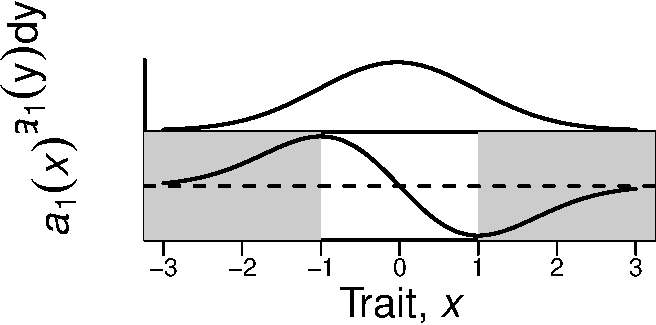
\includegraphics{manuscript_files/figure-latex/fig1-1.pdf}
\caption{The three panels of figure 1, showing examples of evolutionary
landscapes and the corresponding fluctuation domains for three classic
models (logistic, chemostat, branching model). This figure is largely
theoretical, and so easily replicates Figure 1 of the original paper.
The first panel showing the logistic model depicts the fluctuation
regimes for the model parameters used in the numerical analysis.}
\end{figure}

\begin{Shaded}
\begin{Highlighting}[]
\KeywordTok{landscape}\NormalTok{(chemostat_curve, }\DecValTok{1}\NormalTok{, }\DecValTok{9}\NormalTok{)}
\end{Highlighting}
\end{Shaded}

\begin{figure}
\centering
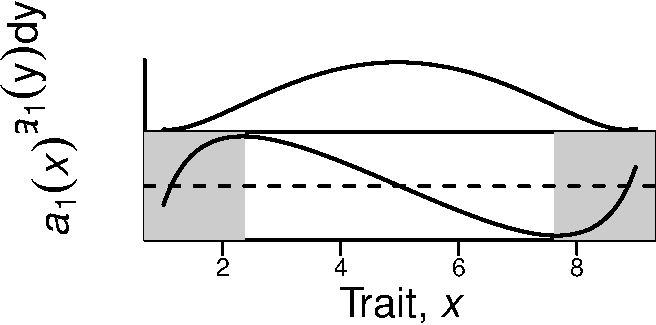
\includegraphics{manuscript_files/figure-latex/fig1-2.pdf}
\caption{The three panels of figure 1, showing examples of evolutionary
landscapes and the corresponding fluctuation domains for three classic
models (logistic, chemostat, branching model). This figure is largely
theoretical, and so easily replicates Figure 1 of the original paper.
The first panel showing the logistic model depicts the fluctuation
regimes for the model parameters used in the numerical analysis.}
\end{figure}

\begin{Shaded}
\begin{Highlighting}[]
\KeywordTok{landscape}\NormalTok{(branching_curve, }\FloatTok{-.8}\NormalTok{, }\FloatTok{.8}\NormalTok{)}
\end{Highlighting}
\end{Shaded}

\begin{figure}
\centering
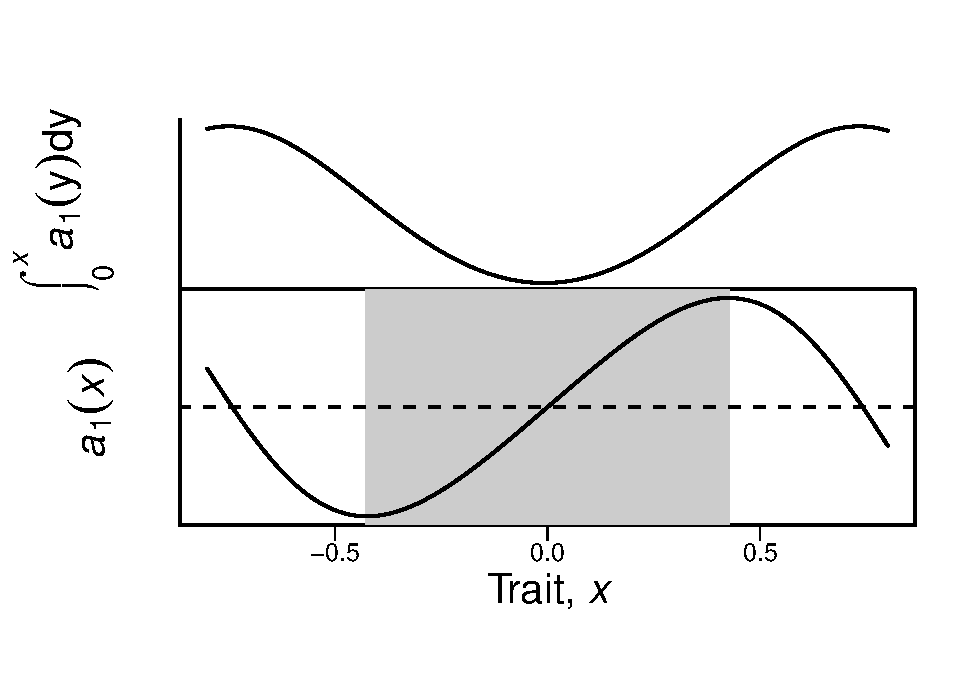
\includegraphics{manuscript_files/figure-latex/fig1-3.pdf}
\caption{The three panels of figure 1, showing examples of evolutionary
landscapes and the corresponding fluctuation domains for three classic
models (logistic, chemostat, branching model). This figure is largely
theoretical, and so easily replicates Figure 1 of the original paper.
The first panel showing the logistic model depicts the fluctuation
regimes for the model parameters used in the numerical analysis.}
\end{figure}

Figure 2 of the original paper has the core computational results
demonstrating the consequences of these fluctuation regimes. The code
for this analysis was implemented as pure C code, which can be run in
stand-alone mode and generates three output text files. The R package
uses the \texttt{.C} interface to pass parameters to the C function
(\texttt{Rlogistic}) which runs the ensemble and writes its output as
text. The C function does not expose a random seed, so re-running the
analysis creates results which are not bitwise identical each time. Of
course the scientific results are expected to be independent of the seed
anyway, so it is perhaps reassuring that as long as the ensemble of
replicates is large enough, the same pattern can be reproduced quite
closely. The original manuscript uses ensembles of 100,000 replicates,
which I have reproduced here. A possible source of confusion is that the
code defaults to only 100 replicates if the ensemble size is not
explicitly verified -- which is an ensemble small enough to still see
random deviations from the predicted results. I probably set that lower
default to facilitate faster testing. Likewise, the MAXTIME parameter
has to be extended from the default setting to allow the third initial
condition set to run sufficiently long.

The code was never parallelized, but runs with a small memory footprint
by streaming simulation data out (e.g.~to disk) over \texttt{fprint}.
Replicating all results takes about an hour of computational time on a
Intel-i7 processor.

\begin{Shaded}
\begin{Highlighting}[]
\NormalTok{out =}\StringTok{ }\KeywordTok{logistic}\NormalTok{(}\DataTypeTok{Xo =} \DecValTok{1}\NormalTok{,  }\DataTypeTok{ENSEMBLES =} \DecValTok{10}\OperatorTok{^}\DecValTok{5}\NormalTok{, }\DataTypeTok{MAX_TIME =} \DecValTok{3000}\NormalTok{)}
\end{Highlighting}
\end{Shaded}

\begin{figure}
\centering
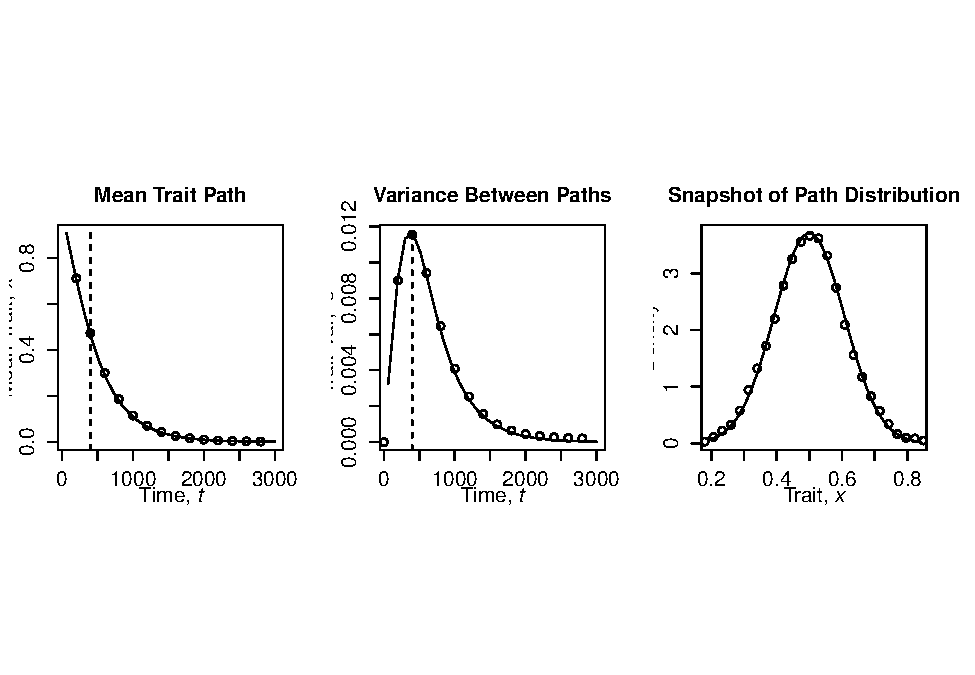
\includegraphics{manuscript_files/figure-latex/unnamed-chunk-2-1.pdf}
\caption{A starting condition of Xo = 1, at the edge of the fluctuation
dissipation regime. The whole evolutionary trajectory thus occurs within
the dissipation regime, and mean dynamics closely match that of the
canonical equation, and show a tight normal distribution around the
expected path. This matches the trajectories seen figure 2 of the
original manuscript.}
\end{figure}

\begin{Shaded}
\begin{Highlighting}[]
\NormalTok{out =}\StringTok{ }\KeywordTok{logistic}\NormalTok{(}\DataTypeTok{Xo =} \DecValTok{2}\NormalTok{,  }\DataTypeTok{ENSEMBLES =} \DecValTok{10}\OperatorTok{^}\DecValTok{5}\NormalTok{, }\DataTypeTok{MAX_TIME =} \DecValTok{5000}\NormalTok{)}
\end{Highlighting}
\end{Shaded}

\begin{figure}
\centering
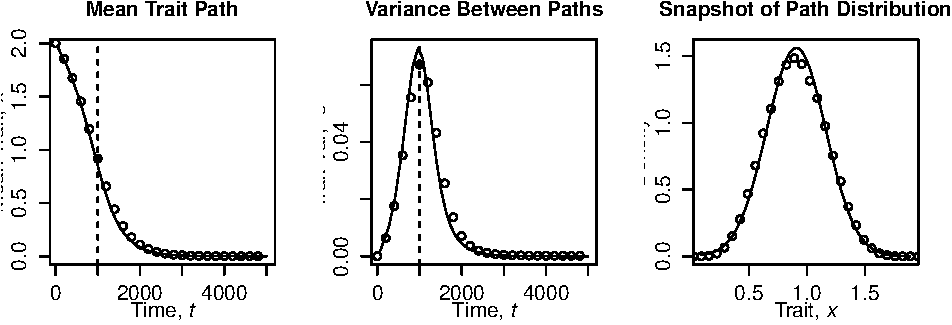
\includegraphics{manuscript_files/figure-latex/unnamed-chunk-3-1.pdf}
\caption{A starting condition of Xo = 2, matching the trajectories seen
figure 2 of the original manuscript. Deviations from the canonical path
are visible, but the distribution is not yet bimodal.}
\end{figure}

\begin{Shaded}
\begin{Highlighting}[]
\NormalTok{out =}\StringTok{ }\KeywordTok{logistic}\NormalTok{(}\DataTypeTok{Xo =} \DecValTok{3}\NormalTok{,  }\DataTypeTok{ENSEMBLES =} \DecValTok{10}\OperatorTok{^}\DecValTok{5}\NormalTok{, }\DataTypeTok{MAX_TIME =} \DecValTok{10000}\NormalTok{)}
\end{Highlighting}
\end{Shaded}

\begin{figure}
\centering
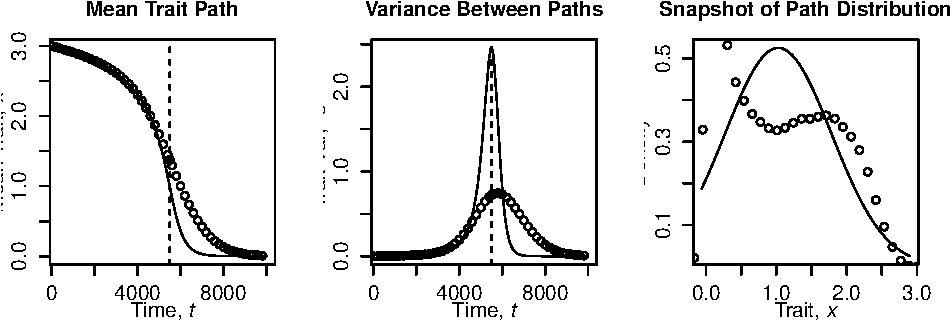
\includegraphics{manuscript_files/figure-latex/unnamed-chunk-4-1.pdf}
\caption{Starting deep in the predicted fluctuation enhancement regime,
Xo = 3, the resulting distribution of trajectories is bimodal, just as
shown in the original figure 2 of the original manuscript.}
\end{figure}

\hypertarget{on-the-r-package-compendium}{%
\subsubsection{On the R package
compendium}\label{on-the-r-package-compendium}}

My original paper acknowledges the use of the R package compendium
approach (Gentleman and Temple Lang 2007) for reproducible research, and
idea later developed in Marwick, Boettiger, and Mullen (2018). While a
decade ago the package as created would pass R's built-in
\texttt{R\ CMD\ check} routine, standards have since evolved and the
current implementation would not do so:

\begin{itemize}
\tightlist
\item
  The C methods are expected to bind R's random number generator
  engines, and not use their own methods, which allows them to
  coordinate with standard R methods for setting seed and so forth.\\
\item
  Data should be passed by reference back to R and not serialized to
  disk (though this can introduce memory constraints).\\
\item
  It is now also standard practice to register the C routines
  explicitly.\\
\item
  \texttt{SystemRequirements} field was not provided in the package
  \texttt{DESCRIPTION}. By adding this to list \texttt{libgsl}, it is
  possible to have the package successfully install on the \texttt{rhub}
  (Csárdi and Salmon 2019) testing platforms.
\end{itemize}

Note that these tighter integrations would also prevent the C libraries
from running as purely stand-alone implementation. In any event, meeting
all the automated checks of a formal package is not an expectation of
the compendium approach, which merely borrows some of the package
tooling.

A dynamic document using RMarkdown (Xie, Allaire, and Grolemund 2018)
for reproducing the present manuscript can be found in the
\texttt{rescience} sub-directory which I have now added to the GitHub
repository housing the original R package,
\url{https://github.com/cboettig/fluctuationDomains}, git tag
\texttt{rescience-submission}, now archived with DOI
\url{https://doi.org/xxxx}.

\hypertarget{conclusions}{%
\section{Conclusions}\label{conclusions}}

In conclusion, I have been able to successfully replicate the original
results. As the original results were not performed with a fixed random
seed, replicated results are statistically comparable but not bitwise
identical. In a scientific sense this is perhaps more useful than
replication with a fixed seed. My compendium approach did not install
entirely out of the box, as an autoconf configure script first required
updating. Ironically, the original version of the code published on a
co-author's personal website and linked from the manuscript both still
existed and did install out-of-the-box. Reproducing the results of the
paper required some careful reading of parameters listed in the paper
and manually knowing what functions to call, as this paper did not
include a complete ``dynamic document'' (Xie 2014, 2015; Xie, Allaire,
and Grolemund 2018) approach discussed in Marwick, Boettiger, and Mullen
(2018) and also used in this replication paper. I think this experience
underscored the critical role dependency management has in frustrating
reproducibility: this replication was relatively simple in part due to
the low number of dependencies and the technical simplicity of the code.
The other take-away for me is how easy it is to leave out small but
important steps needed to reproduce a figure when not using the dynamic
document approach. Despite having R scripts called ``figure1.R'' and
``figure2.R'', these scripts could not simply be run by themselves to
create the figures.

\hypertarget{references}{%
\section*{References}\label{references}}
\addcontentsline{toc}{section}{References}

\hypertarget{refs}{}
\leavevmode\hypertarget{ref-Boettiger2015}{}%
Boettiger, Carl. 2015. ``An Introduction to Docker for Reproducible
Research.'' \emph{ACM SIGOPS Operating Systems Review} 49 (1): 71--79.
\url{https://doi.org/10.1145/2723872.2723882}.

\leavevmode\hypertarget{ref-Boettiger2010}{}%
Boettiger, Carl, Jonathan Dushoff, and Joshua S. Weitz. 2010.
``Fluctuation Domains in Adaptive Evolution.'' \emph{Theoretical
Population Biology} 77 (1): 6--13.
\url{https://doi.org/10.1016/j.tpb.2009.10.003}.

\leavevmode\hypertarget{ref-Boettiger2017}{}%
Boettiger, Carl, and Dirk Eddelbuettel. 2017. ``An Introduction to
Rocker: Docker Containers for R.'' \emph{The R Journal} 9 (2): 527.
\url{https://doi.org/10.32614/RJ-2017-065}.

\leavevmode\hypertarget{ref-rhub}{}%
Csárdi, Gábor, and Maëlle Salmon. 2019. \emph{Rhub: Connect to 'R-Hub'}.
\url{https://CRAN.R-project.org/package=rhub}.

\leavevmode\hypertarget{ref-Dieckmann1996}{}%
Dieckmann, Ulf, and Richard Law. 1996. ``The Dynamical Theory of
Coevolution: A Derivation from Stochastic Ecological Processes.''
\emph{Journal of Mathematical Biology} 34 (5-6): 579--612.
\url{https://doi.org/10.1007/BF02409751}.

\leavevmode\hypertarget{ref-TempleLang2007}{}%
Gentleman, Robert, and Duncan Temple Lang. 2007. ``Statistical Analyses
and Reproducible Research.'' \emph{Journal of Computational and
Graphical Statistics} 16 (1): 1--23.
\url{https://doi.org/10.1198/106186007X178663}.

\leavevmode\hypertarget{ref-Gillespie}{}%
Gillespie, Daniel. 1977. ``Exact Stochastic Simulation of Coupled
Chemical Reactions.'' \emph{Journal of Physical Chemistry} 81.25:
2340--61.

\leavevmode\hypertarget{ref-Marwick}{}%
Marwick, Ben, Carl Boettiger, and Lincoln Mullen. 2018. ``Packaging Data
Analytical Work Reproducibly Using R (and Friends).'' \emph{The American
Statistician} 72 (1): 80--88.
\url{https://doi.org/10.1080/00031305.2017.1375986}.

\leavevmode\hypertarget{ref-renv}{}%
Ushey, Kevin. 2019. \emph{Renv: Project Environments}.
\url{https://CRAN.R-project.org/package=renv}.

\leavevmode\hypertarget{ref-packrat}{}%
Ushey, Kevin, Jonathan McPherson, Joe Cheng, Aron Atkins, and JJ
Allaire. 2018. \emph{Packrat: A Dependency Management System for
Projects and Their R Package Dependencies}.
\url{https://CRAN.R-project.org/package=packrat}.

\leavevmode\hypertarget{ref-knitr}{}%
Xie, Yihui. 2014. ``Knitr: A Comprehensive Tool for Reproducible
Research in R.'' In \emph{Implementing Reproducible Computational
Research}, edited by Victoria Stodden, Friedrich Leisch, and Roger D.
Peng. Chapman; Hall/CRC.
\url{http://www.crcpress.com/product/isbn/9781466561595}.

\leavevmode\hypertarget{ref-knitr_book}{}%
---------. 2015. \emph{Dynamic Documents with R and Knitr}. 2nd ed. Boca
Raton, Florida: Chapman; Hall/CRC. \url{https://yihui.org/knitr/}.

\leavevmode\hypertarget{ref-rmarkdown}{}%
Xie, Yihui, J.J. Allaire, and Garrett Grolemund. 2018. \emph{R Markdown:
The Definitive Guide}. Boca Raton, Florida: Chapman; Hall/CRC.
\url{https://bookdown.org/yihui/rmarkdown}.


\hypersetup{linkcolor=black,urlcolor=darkgray}
\renewcommand\emph[1]{{\bfseries #1}}
\setlength\bibitemsep{0pt}
\printbibliography

\end{document}
